% コンパイル方法: lualatex filename.tex
\RequirePackage{plautopatch}

\documentclass[a4paper, 10pt]{ltjsarticle}


% マージン設定
\usepackage[top=20mm, bottom=20mm, left=20mm, right=20mm]{geometry}

% LuaLaTeX用日本語対応パッケージ
\usepackage{luatexja}
\usepackage{luatexja-fontspec}

% 必要なパッケージ
\usepackage{fontspec}
\usepackage{titlesec}
\usepackage{graphicx}
\usepackage{amsmath}
\usepackage{amssymb}
\usepackage{hyperref}
\usepackage[english, japanese]{babel}
\usepackage{multicol} % 二段組用パッケージ
\usepackage{indentfirst}
\usepackage{tikz} % カスタム点線用
\usepackage{authblk} % 著者・所属パッケージ
\usepackage{here}
\usepackage{caption}
\usepackage{tabularx}
\usepackage{subcaption}

% \setmainfont[Ligatures=TeX]{Times New Roman}
% \setmainjfont[BoldFont=MS Gothic]{MS Mincho}

\renewcommand{\baselinestretch}{0.95}

% セクション見出しのカスタマイズ
\titleformat{\section}
  {\fontsize{10pt}{10pt}}
  {\thesection.}
  {1em}{}

\titleformat{\subsection}
  {\fontsize{10pt}{10pt}}
  {\thesubsection}
  {1em}{}

\titleformat{\subsubsection}
  {\fontsize{10pt}{10pt}}
  {\thesubsubsection}
  {1em}{}

  \setlength{\parindent}{1em}

\captionsetup[table]{skip=0pt}
% \setlength{\belowcaptionskip}{1em} % キャプション下の余白を設定



\titlespacing*{\section}{0em}{1em}{0em}
\titlespacing*{\subsection}{0em}{1em}{0em}

\pagestyle{empty}


\begin{document}

% \setlength{\abovedisplayskip}{1em}
% \setlength{\belowdisplayskip}{1em}
\setlength{\columnsep}{7.5mm}

\twocolumn[
    \begin{center}
        {\vspace{-1em}}

        {\fontsize{15pt}{15pt}\selectfont{クロスレイヤシミュレータにおける無線LAN評価モデルの検討}}

        {\vspace{1.3em}}

        {\fontsize{13pt}{13pt}\selectfont{A Study of a Wireless LAN Evaluation Model in a Cross-Layer Simulator}}
    \end{center}

    \vspace{0.1em}

    \begin{flushright}
      {\fontsize{11pt}{11pt}\selectfont{T5-16 \, 下沢亮太郎}}
      \\
      {\fontsize{11pt}{11pt}\selectfont{指導教員 \, 設樂勇}}
    \end{flushright}

    \vspace{1em}

    \thispagestyle{empty}
]

\section{はじめに}
% 近年,無線通信端末利用者の急増に伴い様々な場所で無線通信システムが利用されており,今後も利用の増加と発展が見込まれている.近年の無線通信技術の進歩に伴い,システムが高機能化・複雑化しており,従来のようにレイヤごとに独立した性能評価を行う手法では通信全体の実用的な評価を十分に行うことが困難になりつつある.そのため,通信全体をクロスレイヤで評価できる計算機シミュレータの開発が求められている.本研究ではクロスレイヤシミュレータにおけるMACレイヤの挙動をシミュレートする機能の開発を行い,その有効性を評価することを目指した.

近年,無線通信端末の利用者が急増し,さまざまな場所で無線通信システムが利用されている.今後もさらなる利用拡大と機能高度化が見込まれる一方,無線通信技術の進歩に伴いシステムが高機能化・複雑化している.従来のように,各レイヤを独立して評価する手法では,通信全体を俯瞰した実用的な性能評価が難しくなりつつある.そのため,物理層から上位層までを跨いで統合的に評価できるクロスレイヤシミュレータの開発が求められている.本研究では,クロスレイヤシミュレータの一部としてMACレイヤの挙動をシミュレートする機能を開発し,その有効性を評価することを目的とする.


\section{研究背景}
一般的な無線通信分野における評価・解析は各レイヤごとに独立して行われており,物理層からアプリケーション層までのレイヤを跨いだ通信全体の一貫的な評価を行うことができない.また,従来手法ではマルコフ連鎖モデルを用いて評価することが多かったが,本研究では\texttt{Python}を用いて開発することで,新規の通信プロトコルの検証を容易に組み込み検証できるクロスレイヤシミュレータの開発を目指す.



\section{無線LAN通信モデル}

本研究では,IEEE 802.11規格に基づく無線LAN通信を再現するために,CSMA/CA(Carrier Sense Multiple Access with Collision Avoidance)方式を用いたモデルを開発した.

\subsection{CSMA/CA}

IEEE 802.11規格では,CSMA/CAと呼ばれる方式を採用している.これは,送信前にチャネルが空いているかを確認し,空いていれば送信を試みる手法である.図\ref{CSMA/CA}にCSMA/CAの概要を示す.

CSMA/CAでは,端末が送信チャネルをキャリアセンスし,チャネルが空いているときにパケット送信を行う.一方,チャネルが使用中であれば一定時間バックオフを行う.バックオフ期間中は端末ごとにランダムにスロット数を生成し,それに従って待機することで他端末との衝突を回避する.複数の端末が同じスロット数を生成した場合には送信タイミングが重なり,衝突が発生するため再送処理が必要となる.


\begin{figure}[H]
  \centering

  \begin{subfigure}{\columnwidth}
    \centering
    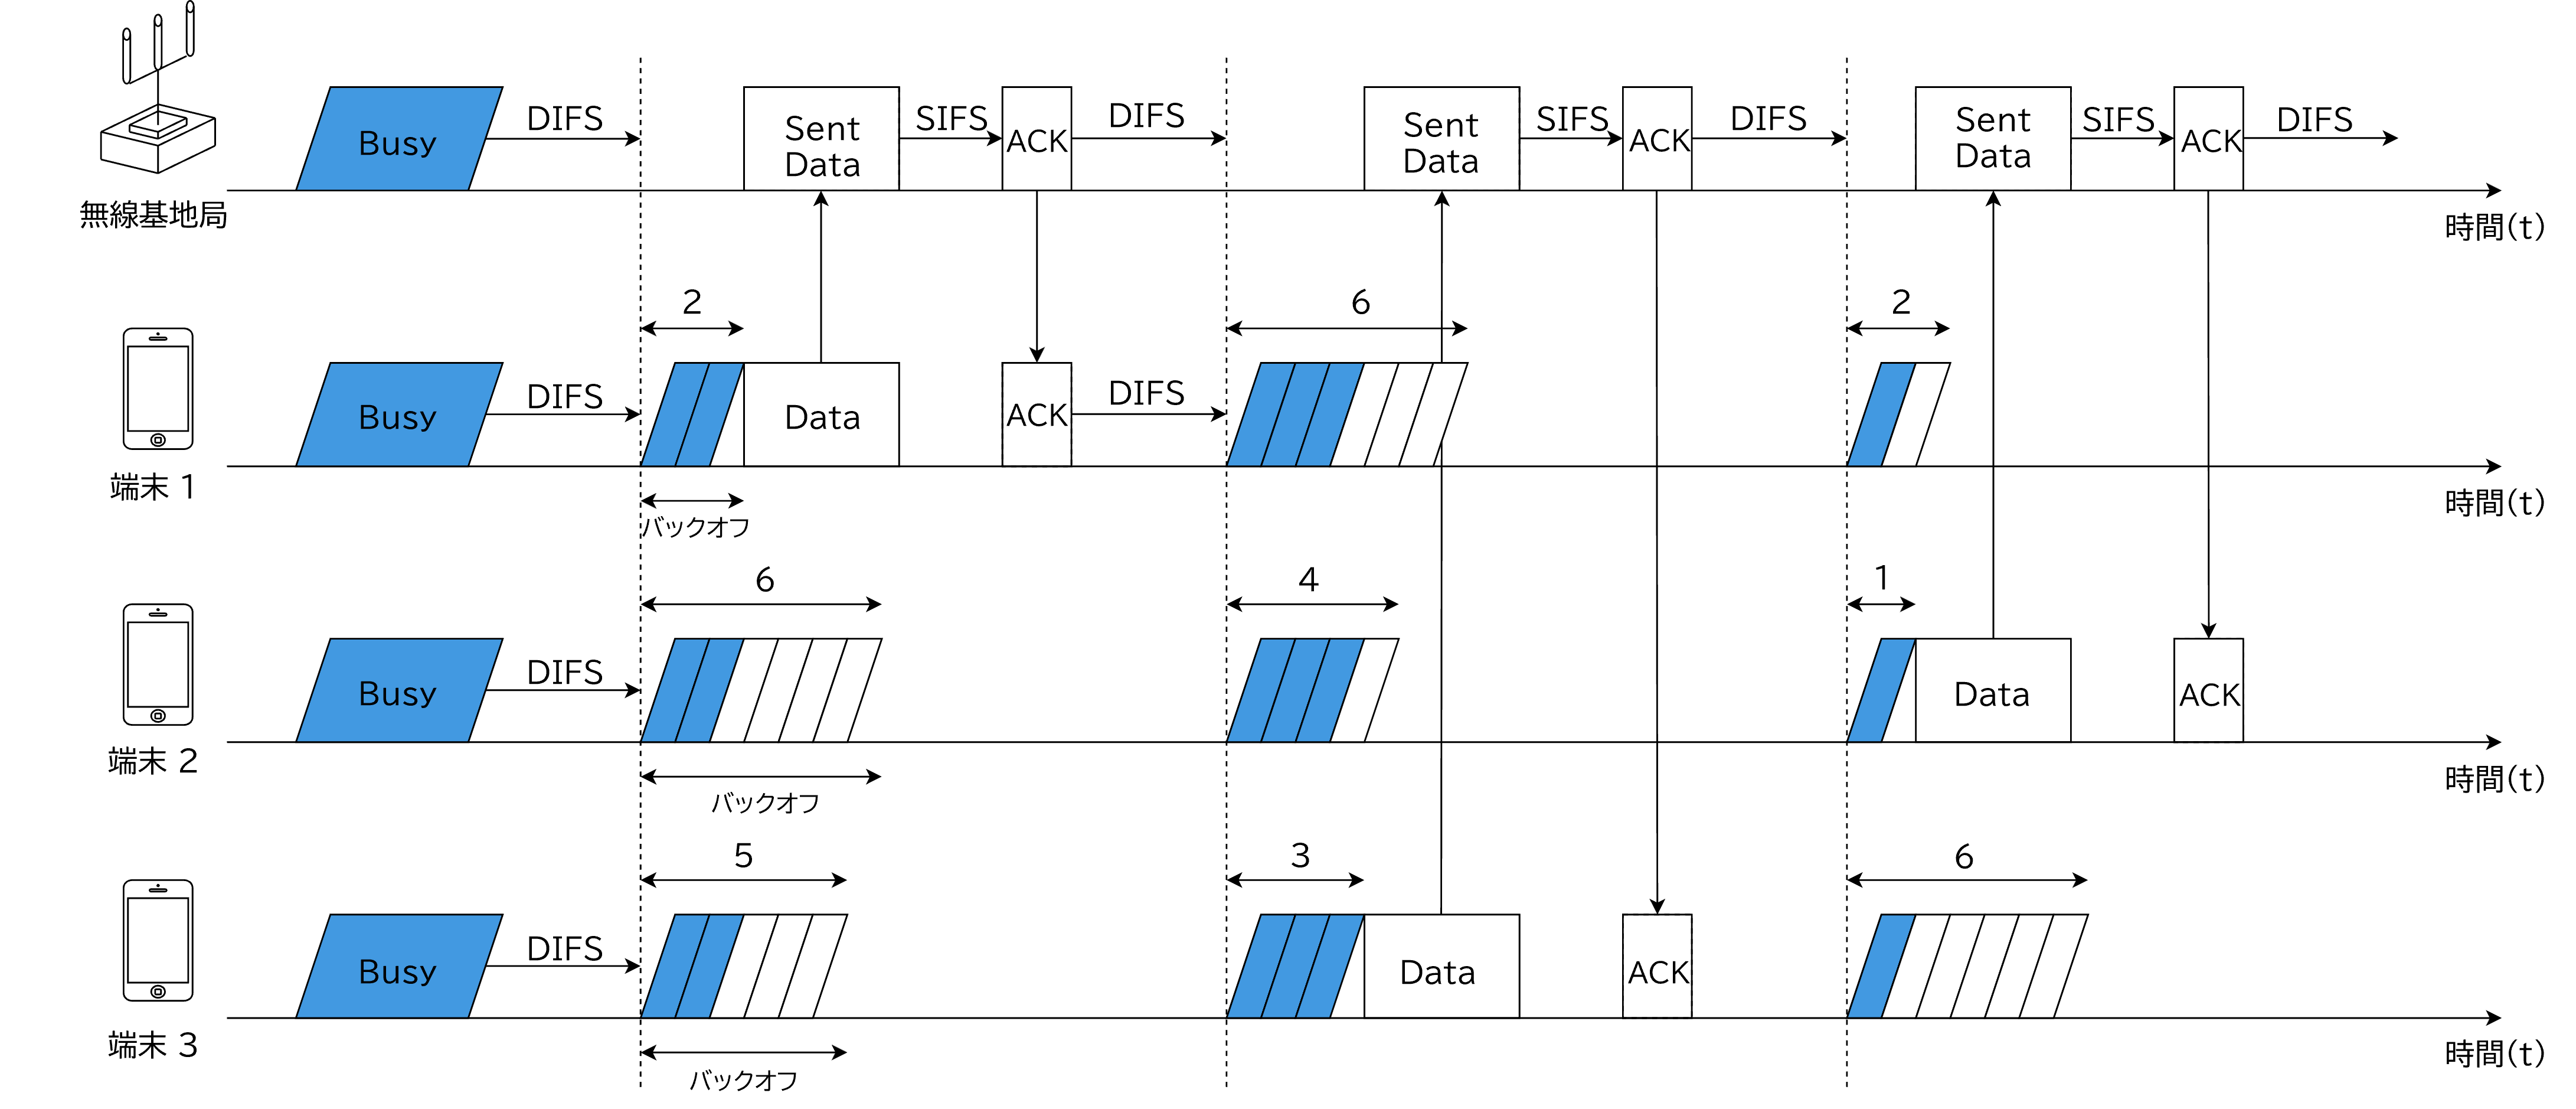
\includegraphics[width=1\columnwidth]{./assets/csma-ca-s.png}
    \caption{CSMA/CA成功例}
  \end{subfigure}


  \begin{subfigure}{\columnwidth}
    \centering
    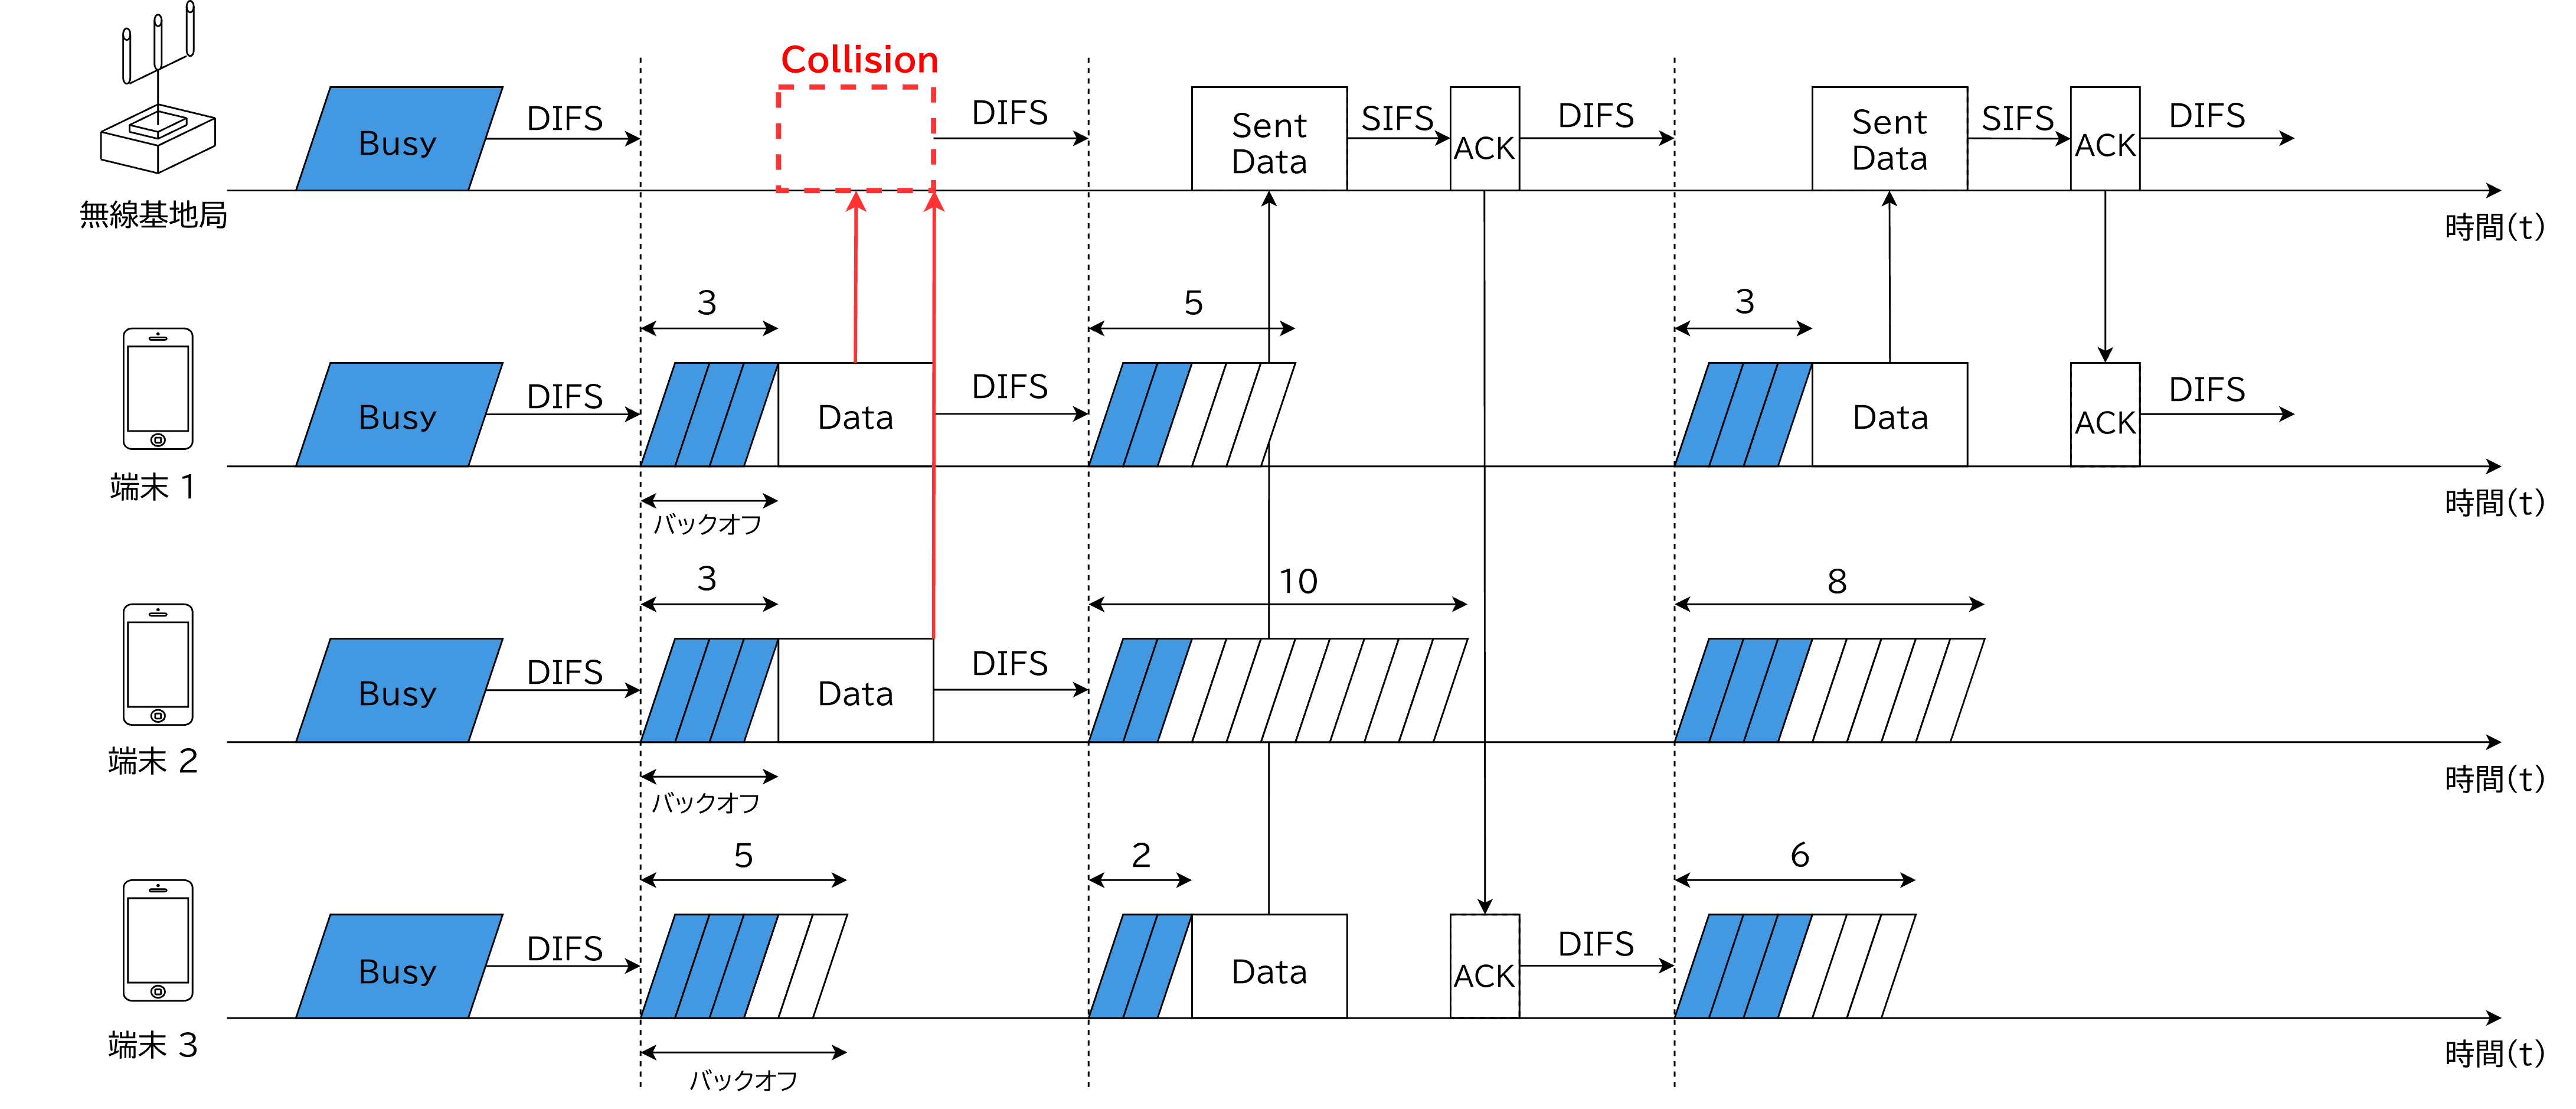
\includegraphics[width=1\columnwidth]{./assets/csma-ca-f.png}
    \caption{CSMA/CA失敗例}
  \end{subfigure}
  % 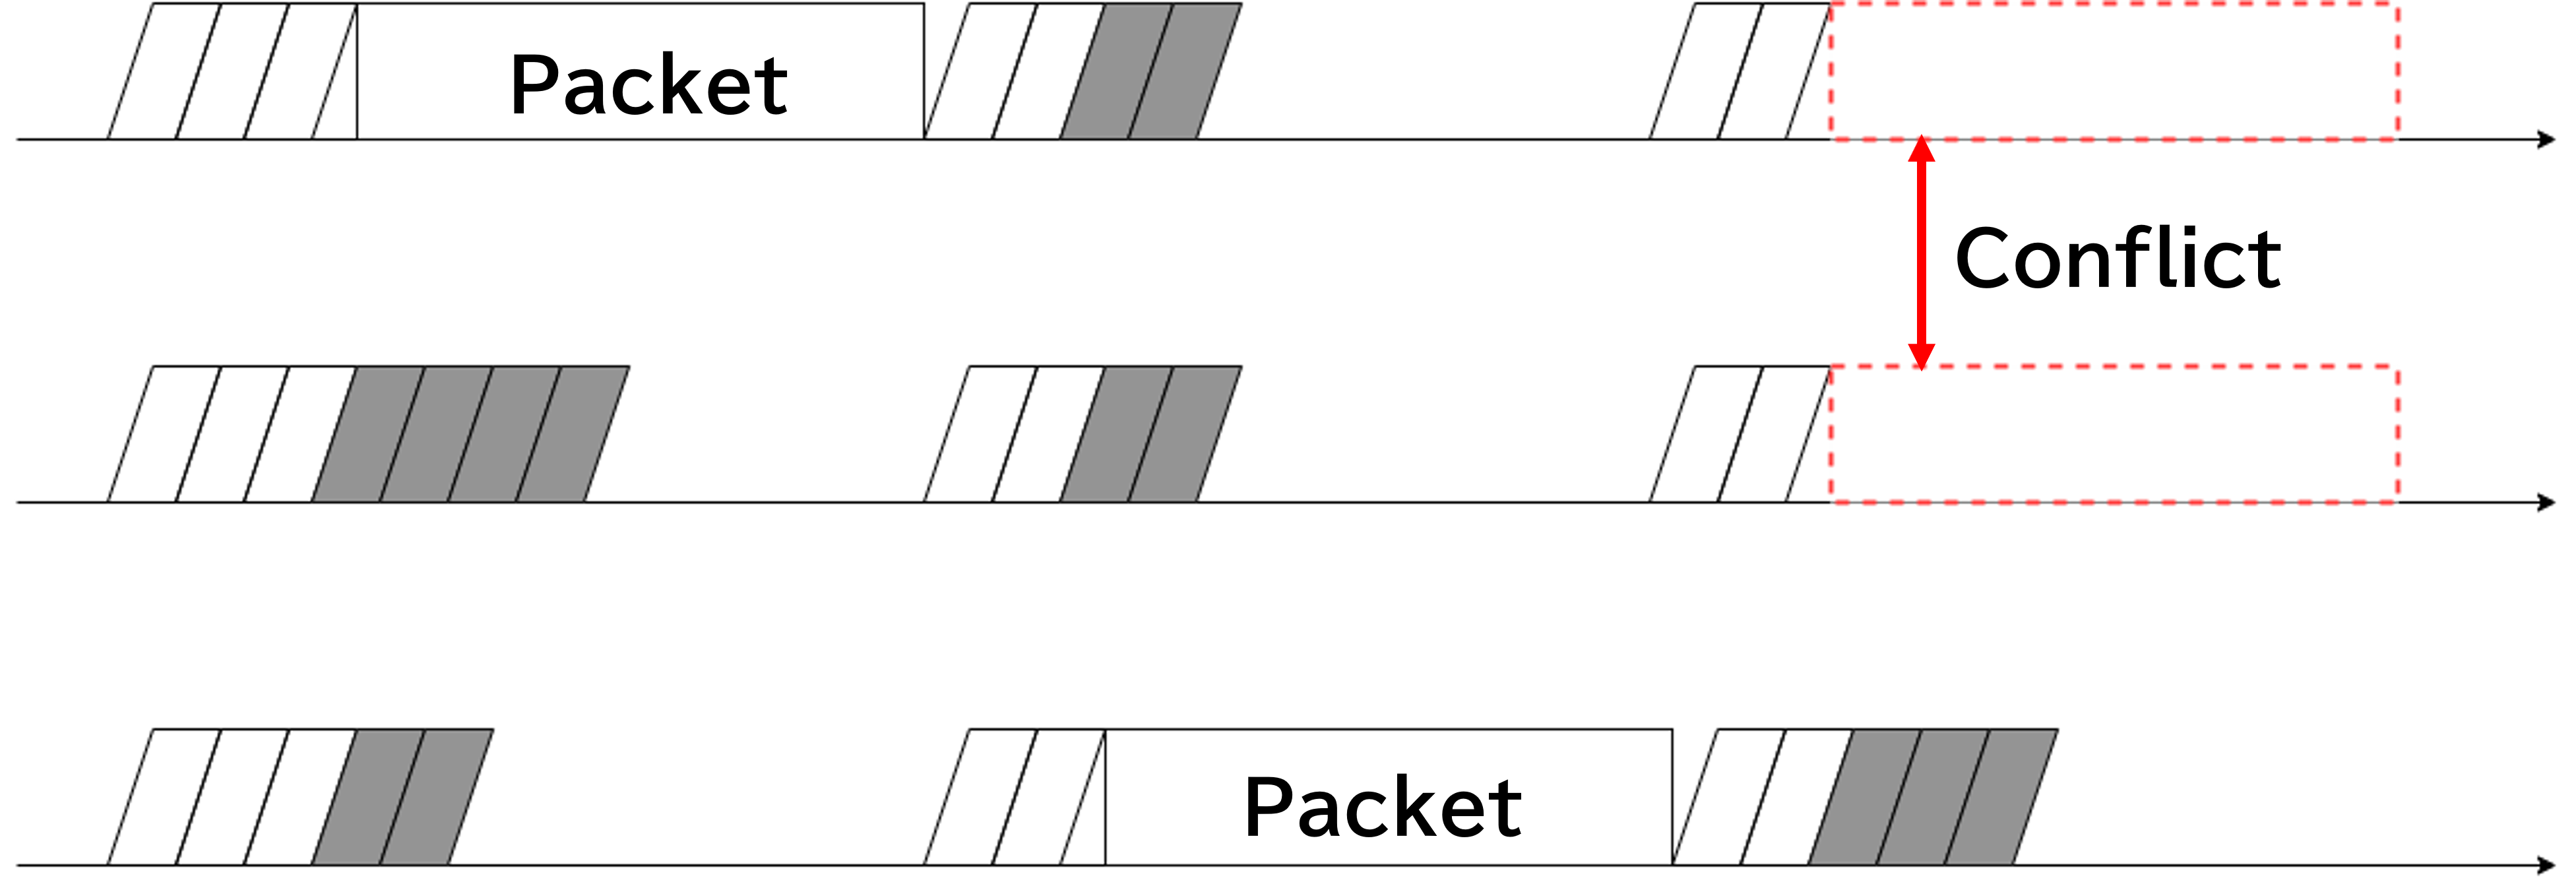
\includegraphics[width=1\columnwidth]{./assets/csmaca-1.png}
  % \caption{CSMA/CA概要図}
  \label{CSMA/CA}
\end{figure}

\subsubsection{CW(Contention Window)}

バックオフ時に用いるコンテンションウィンドウは,最大値の上限を1023スロットとして衝突回数や再送制御のパラメータに応じて変化する.

再送回数を$n$とするとCWの最大値は


% 再送回数を$n$とするとCWの最大値は

\begin{align}
  \text{cw\_max} &= 2^{4 + n} - 1
\end{align}

となる.さらに,スロット数$s$は

\begin{align}
  s &= \mathrm{randint}(1, \, \min(\text{cw\_max}, \, 1023))
  \label{slot}
\end{align}

で求められる.

本研究では,上記の式を用いて各端末が送信を試みる際の待機時間(スロット数)を動的に設定する処理を実装した.CSMA/CAによるランダムアクセスは,衝突の確立が低下し,再送できる回数が増えるが,バックオフ時間の増加による遅延が発生し,スループットが低下する可能性がある.

\subsection{パケット構成モデル化}
% UDPレベルでの無線LAN通信をシミュレートするために,簡易的にパケットを構成するモデルを作成した.図\ref{packet}に,モデル化されたパケットの構成図を示す.

本研究では,UDPレベルの無線LAN通信を再現するためにPLCPプリアンブル,MACヘッダー,FCS等のプリアンブルやフッタ,オーバーヘッドを含めたパケット構成を簡易的にモデル化した.図\ref{packet}にモデル化したパケットの構成図を示す.





\begin{figure}[H]
  \centering
  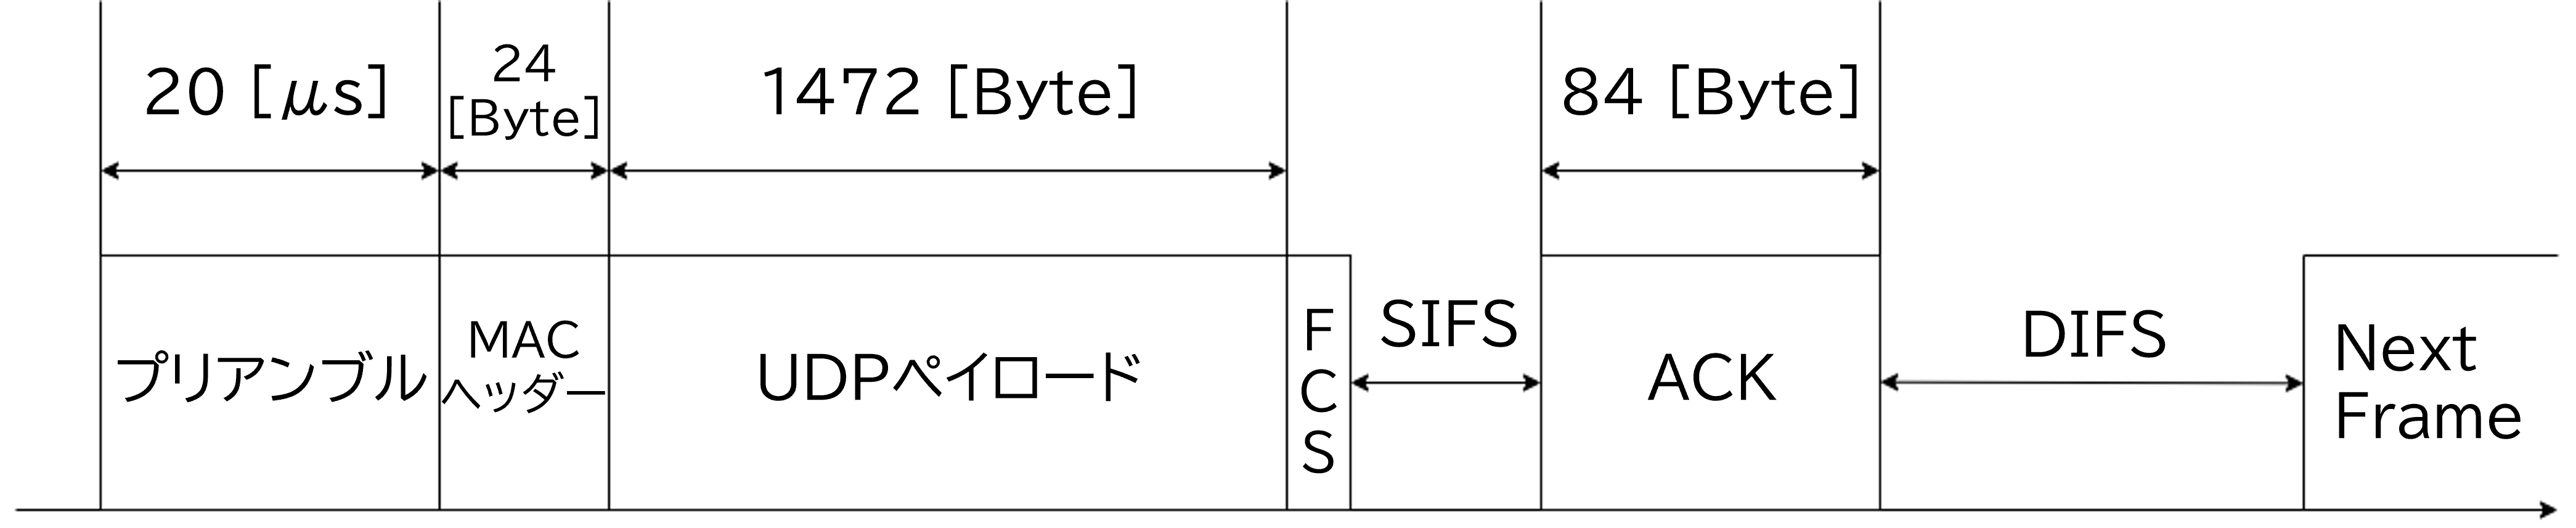
\includegraphics[width=1\columnwidth]{./assets/packet.png}
  \caption{モデル化されたパケット構成図}
  \label{packet}
\end{figure}


% \section{提案手法}
% \subsection{User class}

\section{実装とシミュレーション設定}

本研究では,CSMA/CA方式を用いた無線LAN通信を再現するために,Pythonを用いてシミュレータを実装した.シミュレータの主な機能として,端末ごとのCWや再送回数の管理,スロット数の動的な設定,再送処理などを実装した.

また,シミュレータ本体は標準ライブラリである\texttt{random}のみに依存するように設計し,他のライブラリに依存しないようにした.これにより,バージョンに依存しづらい後方互換性が保たれたシミュレータを実装することができた.


\subsection{\texttt{User}クラスの設計}
本研究のシミュレータ実装では、各端末を\texttt{User}クラスとして定義し、端末ごとのCWや再送回数などを管理している.表\ref{tab:user-class}に主なメンバ変数と役割をまとめる.

% \begin{table}[H]
%   \centering
%   \caption{Userクラスのメンバ変数とメソッドの一覧}
%   \label{tab:user-class}
%   \begin{tabularx}{\columnwidth}{lX}
%     \hline
%     % \textbf{名称} & \textbf{説明} \\
%     名称 & 説明 \\
%     \hline
%     \multicolumn{2}{l}{メンバ変数} \\
%     \hline
%     \texttt{id} & 端末を識別するためのID\\
%     \texttt{num\_re\_trans} & 再送回数\\
%     \texttt{slots} & スロット数\\
%     \texttt{num\_transmitted} & 送信成功回数\\
%     \texttt{data\_transmitted} & 送信したデータ量 \, [bit]\\
%     \hline
%     \multicolumn{2}{l}{主なメソッド} \\
%     \hline
%     \texttt{calc\_slots()} &(\ref{slot})式に従い\texttt{slots}を決定\\
%     \texttt{re\_transmit()} & 再送処理\\
%     \texttt{reset\_slots()} & 新たに\texttt{slots}を割り当てる\\
%     \hline
%   \end{tabularx}
% \end{table}

\subsection{シミュレーションパラメータ}
表\ref{tab:sim-param}に,本研究で用いシミュレーションパラメータを示す.規格(IEEE 802.11a/b/g)によりスロット時間やDIFS/SIFSなどのタイミングパラメータが異なるため,対応するモードを選択することで,より実環境に近い動作を再現できる.


\begin{table}[H]
  \centering
  \caption{シミュレーションパラメータの例}
  \label{tab:sim-param}
  \begin{tabular}{|c|@{\hspace{1.8em}}l|}
    \hline
    パラメータ & 値・例 \\
    \hline
    シミュレーション時間 & 60 \, [$\mathrm{s}$] \\
    スロット時間 (802.11a) & 9 \, [$\mathrm{\mu s}$] \\
    DIFS (802.11a) & 34 \, [$\mathrm{\mu s}$] \\
    SIFS (802.11a) & 16 \, [$\mathrm{\mu s}$] \\
    伝送レート & 24 \, [Mbps] \\
    端末数 & 80 \, [台] \\
    \hline
  \end{tabular}
\end{table}


\section{評価}
図\ref{fig:simulation-result}に,横軸を端末数,縦軸をスループットとしてプロットしたシミュレーション結果と理論値を示す.


\begin{figure}[H]
  \centering
  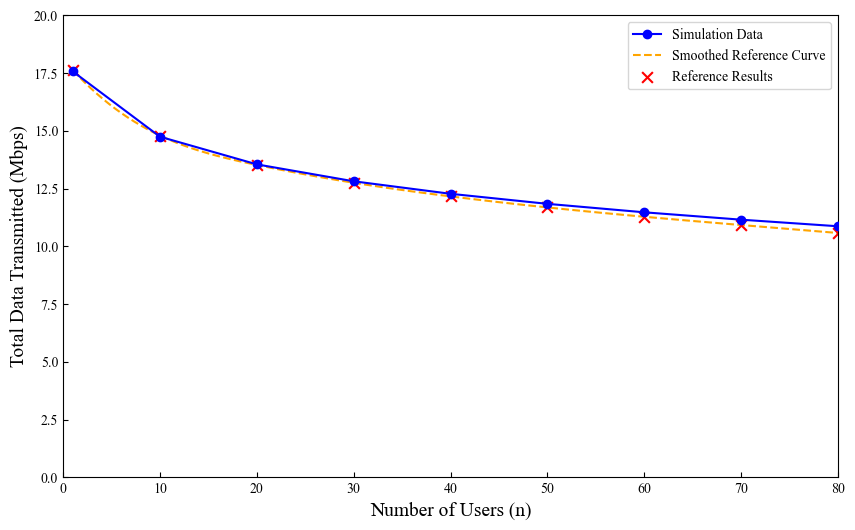
\includegraphics[width=1\columnwidth]{./assets/g3.png}
  \caption{シミュレーション結果}
  \label{fig:simulation-result}
\end{figure}


理論値との差が一番大きい端末数が80台の場合でも+2.75\%程度の誤差に収まっていることがわかる.

また,端末数が増加するにつれて理論値との差が徐々に拡大することに対しては,参考とした文献\cite{paper}とのモデル化方法の違いが影響していると考えられる.

\section{結言}
本研究では,クロスレイヤシミュレータの一部として無線LAN通信の挙動を再現するシミュレータを開発し,CSMA/CAを中心とした基本動作のモデル化とその有効性を検証した.

今後の課題としては,連続送信ではなくポアソン分布などに従った送信間隔を導入することで実際の通信頻度に近い状況を再現することや,端末間の距離による自由空間伝搬損失などの要素を考慮し,より実環境に近い評価を行う必要がある.


% 本研究では,クロスレイヤシミュレータの一部である無線LANシミュレータを開発し,CSMA/CAを中心とした動作のモデル化と検証を行った.

% また,現在の方法では通信が連続して行われているが,ポアソン分布に従った時間だけ離すことで実際の通信頻度に近い状況を再現することや,各ステーションに距離の概念を持たせて自由空間伝搬による減衰を考慮することが今後の課題である.

\begin{thebibliography}{9}
  \bibitem{midori}守倉正博, 久保田周治, 『インプレス標準教科書シリーズ 改訂三版802.11 高速無線LAN教科書』, 株式会社インプレスコミュニケーションズ, 2016年
  \bibitem{paper}Y. Morino, T. Hiraguri, H. Yoshino, K. Nishimori, T. Matsuda, ``A Novel Collision Avoidance Scheme Using Optimized Contention Window in Dense Wireless LAN Environments*'' \, \textit{IEICE TRANS. COMMUN.}, VOL.E99-B, NO.11 NOVEMBER 2016
\end{thebibliography}



\end{document}
